\documentclass[]{article}

\usepackage{url}
\usepackage{tikz}
\usepackage{graphicx}

\title{Demonstration of how to include Tikz and Inkscape images in a \LaTeX document}
\author{Tom Ravalde}
\date{\today}

\begin{document}

\maketitle

Here are examples of how to include graphics in a \LaTeX document, using the Tikz package, or the Inkscape vector graphics editor.

\section{Tikz}

Figure~\ref{fig:tikz} shows an image made using the Tikz package. To see the commands, take look at the \TeX source for this document. There are lots of templates for different sorts of diagrams (e.g. flowcharts, 3D shapes, mindmaps etc.) at \url{http://www.texample.net/tikz/examples/all/}.

\begin{figure}
  \centering

  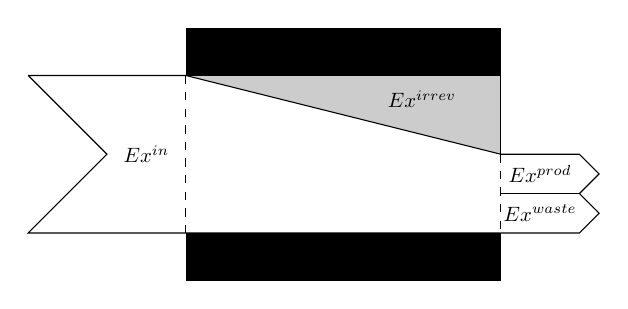
\begin{tikzpicture}

    % Black box
    \draw[fill=black] (-2,-1.6) -- (2,-1.6) -- (2,1.6) -- (-2,1.6); 

    % Irreversibility rectangle
    \draw[fill=black!20] (-2,-1) -- (2,-1) -- (2,1) -- (-2,1); 

    % Xxergy flow
    \draw[fill=white] (-4,1) -- (-2,1) -- (2,0) -- (3,0) --(3.25,-0.25) -- (3,-0.5) -- (3.25,-0.75) -- (3,-1) -- (2,-1) -- (-2,-1) -- (-4,-1) -- (-3,0) -- (-4,1); 

    % black box lines (LHS)
    \draw[dashed, fill=white] (-2,1) -- (-2,-1) ; 

    % black box lines (RHS)
    \draw[dashed, fill=white] (2,0) -- (2,-1) ;

    % Separate product and waste
    \draw[fill=white] (2,-0.5) -- (3,-0.5) ; 

    % Include text at appropriat locations
    \node[scale=0.75] at (-2.5,0) {$Ex^{in}$};
    \node[scale=0.75] at (1,0.7) {$Ex^{irrev}$};
    \node[scale=0.75] at (2.5,-0.25) {$Ex^{prod}$};
    \node[scale=0.75] at (2.5,-0.75) {$Ex^{waste}$};
  \end{tikzpicture}
  \caption{An image created using the Tikz package.}
  \label{fig:tikz}

\end{figure}

\section{Inkscape}

This is now my preferred method. It's generally easier, and yet the output quality is equivalent to Tikz, if you get it right.

\begin{enumerate}
    \item Draw your image in Inkscape. Include text using a text box. For text, type is if you are writing directly into \LaTeX, so for example you can enclose text inside \verb $ ~signs for mathematics, or use commands such as \verb \textbf ~etc.
    \item Save your image in SVG (scale-vector graphics format). This will be the version you edit. Here, the image is saved as \texttt{image.svg}.
    \item The next step is to convert your Inkscape SVG into two separate files:
    \begin{enumerate}
	\item A PDF file, which will be all the non-text components of your SVG image (e.g. \texttt{image.pdf})
	\item A pdf\_tex file, which will be TeX code which imports the PDF image, and adds the text in the correct location (e.g. \texttt{image.pdf\_tex}). This makes the text consistent with the font and options, as defined for the rest of the document.
    \end{enumerate}

    There are two ways to create these files -- one more manual, the other more nerdy. Once they have been created, you can include the image in the document using \verb \input{image.pdf_tex} ~within a figure environment, as in Figure~\ref{fig:inkscape}.
\end{enumerate}

\begin{figure}
    \centering
    \includegraphics[width=0.5\textwidth]{pdf-save}
    \caption{Saving an Inkscape SVG image to the appropriate format.}
    \label{fig:saving}
\end{figure}

\subsection{The manual method}

In Inkscape, use the File menu to saveas a PDF. A box will come up allowing you to set some options. Tick the checkbox which says \texttt{PDF+LaTeX: Omit text in PDF, and create LaTeX file} (Figure~\ref{fig:saving}). Then click okay, and this will create both the PDF and the pdf\_tex file.

\begin{figure}
    \centering
%\def\svgwidth{\textwidth}{\input{image.pdf_tex}}
    \resizebox{\columnwidth}{!}{\input{image.pdf_tex}}
    \caption{An image created as an SVG using Inkscape, and included into a LaTeX document.}
    \label{fig:inkscape}
\end{figure}

\subsection{The nerdier method}

If you prefer to work at a UNIX-based command line (either directly, or by using a bash script, or Makefile), then you can convert the SVG file to the PDF and pdf\_tex files with the following command:

\begin{verbatim}
inkscape -D -z --file=image.svg --export-pdf=image.pdf --export-latex
\end{verbatim}

\end{document}
